\begin{figure}
	\centering
	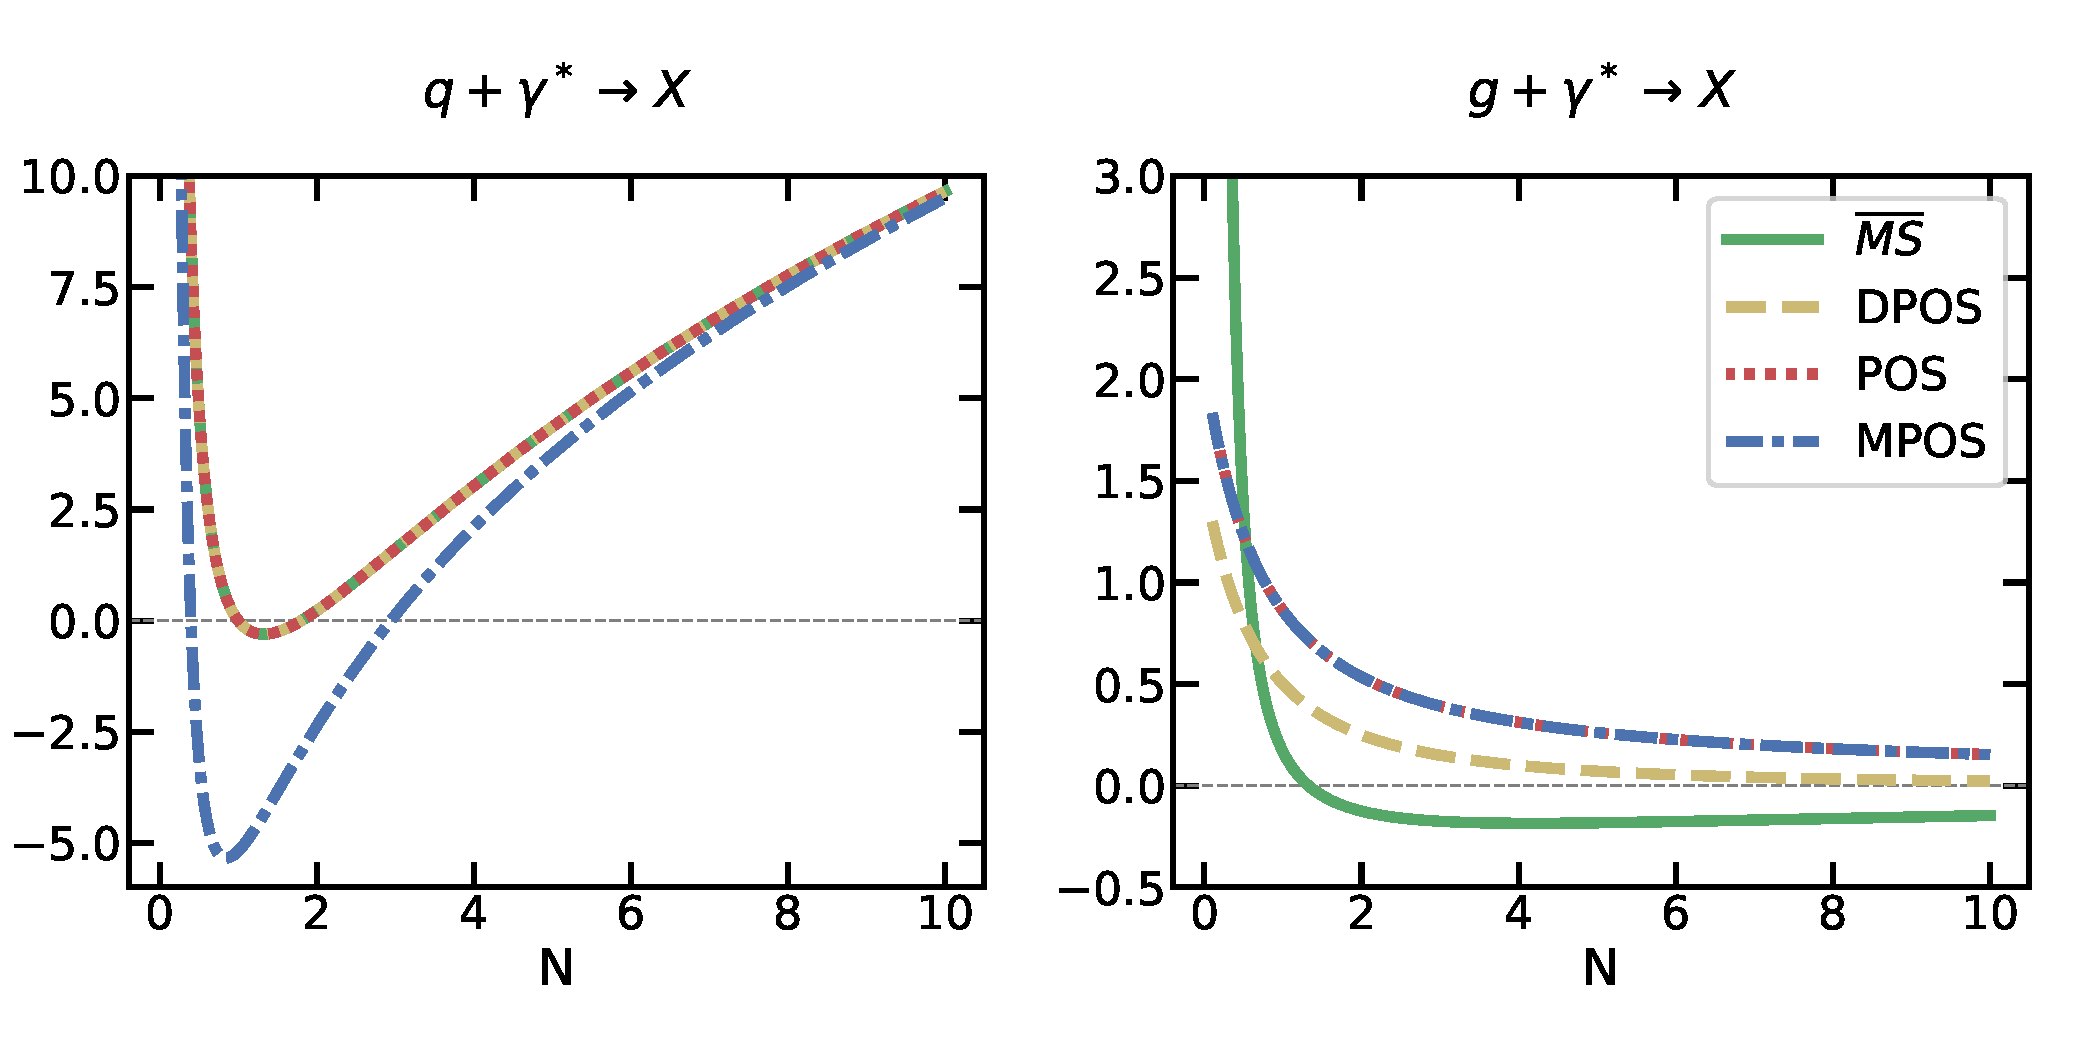
\includegraphics[width=0.7\textwidth]{ch-qcd/dis}
	\caption{The \acrfull{dis} process.}
	\label{fig:qcd/dis}
\end{figure}

The Deep Inelastic Scattering process is the scattering of a lepton over an
hadron component, mediated by an \ew boson \cref{fig:qcd/dis}.
%
The leptonic part does not couple directly to \qcd , thus the $\alpha_s$
corrections do apply only to the hadronic side (at \lo \ew), and the \ew boson
can be seen as emitted from the incoming lepton and absorbed into the hadron.
%
In this picture the process can be interpreted as the scattering of an
off-shell \ew boson over an hadron, probing the hadron composition.
